\section{Introduction}\label{sec:introduction}

The Colin de Verdière invariant connects graph colouring with the
inertia and nullity of real symmetric matrices. We prove that the
chromatic number need not be at most one more than this invariant.

\subsection{The invariant and the main result}

A real symmetric matrix \(M\), indexed by the vertices of a finite
nonempty simple graph \(G=(V,E)\), is \emph{well-signed for \(G\)} if, for
distinct vertices \(u,v\),
\[
 M_{uv}<0\quad\text{when }\{u,v\}\in E,\qquad
 M_{uv}=0\quad\text{when }\{u,v\}\notin E.
\]
Its diagonal entries are unrestricted. Such a matrix has the
\emph{Strong Arnold Property} if the only real symmetric matrix \(X\)
satisfying
\[
 MX=0,\qquad X_{uu}=0\ (u\in V),\qquad
 X_{uv}=0\ (\{u,v\}\in E)
\]
is \(X=0\). The Colin de Verdière invariant is
\[
 \mu(G)=\max\left\{\dim\ker M:\ 
 \begin{array}{l}
 M\text{ is well-signed for }G,\quad n_-(M)=1,\\
 M\text{ has the Strong Arnold Property}
 \end{array}\right\},
\]
where \(n_-(M)\) counts negative eigenvalues with multiplicity.
This class is nonempty: perturb an invertible diagonal matrix with
one negative entry by sufficiently small negative entries on the
edges. Inertia and invertibility persist, and an invertible matrix
has the Strong Arnold Property.

Write \(\alpha(G)\) and \(\chi(G)\) for the independence number and
chromatic number. The chromatic conjecture for this invariant asserts
that \(\chi(G)\le\mu(G)+1\) for every finite nonempty simple graph.
Our main result gives a negative resolution.

\begin{theorem}\label{thm:main}
There are finite graphs \(G\) of arbitrarily large order for which
\[
 \alpha(G)\le2,\qquad
 \mu(G)+1<\frac{|V(G)|}{2}\le\chi(G).
\]
In particular, the Colin de Verdière chromatic conjecture is false.
\end{theorem}

We prove a stronger matrix obstruction than is necessary for the
upper bound on \(\mu\): every well-signed matrix on the constructed
graph with one negative eigenvalue has rank greater than
\(|V(G)|/2+1\). The Strong Arnold Property is not used in this bound.
The maximum corank in this larger class is the related parameter
\(\kappa\) considered by Lovász and Schrijver
\citep[pp.~572--574]{lovaszschrijver2017}. Thus the construction also
satisfies \(\kappa(G)+1<|V(G)|/2\). Unlike \(\mu\), this larger
parameter is not minor-monotone in general; our argument uses it only
through the stated matrix class.

\subsection{History, significance, and the construction}

Colin de Verdière introduced \(\mu\) through the spectral study of
Schrödinger operators on graphs \citep{cdv1990,hls1999}.
The Strong Arnold Property expresses a transversality condition from
that spectral framework \citep{cdv1988arnold}. The small values of the
invariant have concrete geometric meanings: \(\mu\le2\) characterizes
outerplanar graphs, \(\mu\le3\) planar graphs, and \(\mu\le4\)
linklessly embeddable graphs \citep{cdv1990,lovaszschrijver1998,hls1999}.
The proposed chromatic bound holds throughout the range
\(\mu(G)\le4\) \citep[p.~35]{hls1999}.
Gram representations and nullspace embeddings have provided geometric
ways to study these matrices \citep{kotlovlovaszvempala1997,lovaszschrijver1999}.
These connections make the proposed chromatic bound a natural test of
how much colouring information the spectral invariant retains.

Write \(h(G)\) for the largest \(t\) such that \(K_t\) is a minor of
\(G\). Minor monotonicity of \(\mu\), together with
\(\mu(K_t)=t-1\), gives \(h(G)\le\mu(G)+1\)
\citep[\S1.3 and Theorem~2.4]{hls1999}. Thus Hadwiger's conjecture
\(\chi(G)\le h(G)\) \citep{hadwiger1943} would imply the chromatic
bound proposed by Colin de Verdière \citep{cdv1990,cdv1998,hls1999}.
For completeness, the complete-graph identity follows directly from
\(-J_t\): it has one negative eigenvalue and nullity \(t-1\), and the
Strong Arnold Property is automatic on a complete graph. No admissible
matrix can have rank zero. The examples in \Cref{thm:main} therefore
also violate Hadwiger's inequality. The matrix obstruction below is
proved directly; its conclusion does not follow from a clique-minor
obstruction.

A distinct connected-matching route to the failure of Hadwiger's inequality
is given in the companion manuscript~\citep[Theorem~1.1 and Corollary~1.2]{OpenAIHadwigerCounterexample2026}.

The construction starts with a finite-field relation of \emph{holes}.
Its vertices are injective frames. A hole is witnessed by a tensor
shared by two frames, two compatible affine-gradient equations, and a
parity condition. Summing those equations around a triangle gives a
contradiction. The complement of the hole relation consequently has
independence number at most two, and so needs at least half its order
in colours. Our remaining task is to force matrix rank strictly above
half the order. For this purpose, ordinary control of connected
matchings is insufficient: the matrix argument needs conflicts between
specified classes of matching edges and between a matching and a
separately chosen vertex set.

The new probabilistic ingredient is a thinning of the allowed
channel images that preserves the primal-frame distribution. It
penalizes prescribed nonzero translates of channel combinations,
turning the difficult phase alternative into one with a fixed
positive mass of compatible pairs. This gives both a version of
conflict supersaturation that distinguishes colours and an
asymmetric edge--point version. We prove these extensions together
with their common-limit and finite-sampling steps. The low-rank Boolean
moment argument uses commuting multiplication operators, as in the
flat-extension method for moments \citep{laurentmourrain2009}; here the
characteristic-two, partly truncated version is proved directly. The
probabilistic comparison combines entropy control with the
energy-increment method of weak regularity \citep{cover2006,frieze1999}.
For finite sampling we adapt the deterministic fingerprint procedure of
Kleitman and Winston \citep{kleitmanwinston1982,samotij2015}, using a
constrained entropy minimum as its potential \citep{csiszar1975}.

The second ingredient is a matrix criterion for clique blow-ups.
A finite-tree representation of hyperbolic flats locates large
families of blocks that can be normalized simultaneously. A first
spectral normalization produces an almost perfect matching of
coordinates. A second normalization extracts additional positive
directions from selected pair blocks. The resulting rank gain
contradicts a kernel of approximately half the total dimension.
The criterion needs only the graph properties stated next and
may be used independently of the tensor construction.

\subsection{The base graphs and the proof structure}

A \emph{hole} of a graph is a pair of distinct nonadjacent vertices.
Two edges \emph{conflict} if they are disjoint and all four cross
pairs between their endpoints are holes. An edge and a vertex
conflict if the vertex is distinct from both endpoints and both
cross pairs are holes. Edges \emph{touch} if they have a common
endpoint or an edge joins their endpoint sets. Thus two disjoint
edges fail to touch exactly when they conflict.



\noindent\begin{minipage}{\linewidth}
\begin{theorem}[Base graphs]\label{thm:base-graphs}
There is a constant \(a>0\) such that, for every \(\beta>0\),
there are arbitrarily large integers \(m\) and graphs \(H\) on
\(m\) vertices with \(\alpha(H)\le2\) and the following properties.
\begin{enumerate}[label=\textup{(G\arabic*)},ref=G\arabic*]
\item\label{item:base-colours}
Every matching of size at least \(m/20\), partitioned into classes
of size at most \(am\), contains two conflicting edges in different
classes.
\item\label{item:base-edge-point}
Every matching of size at least \(\beta m\) and every vertex set
of size at least \(\beta m\) contain an edge and a vertex in conflict.
\item\label{item:base-holes}
Every two vertex sets of size at least \(\beta m\) contain a cross
hole.
\end{enumerate}
The two vertex sets in \ref{item:base-holes} may overlap.
\end{theorem}
\end{minipage}\par

\begin{figure}[htbp]
\centering
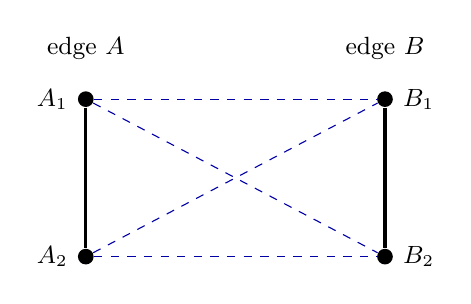
\begin{tikzpicture}[scale=1.0,every node/.style={font=\small}]
\node[circle,fill=black,inner sep=2pt,label=left:\(A_1\)] (a1) at (0,1) {};
\node[circle,fill=black,inner sep=2pt,label=left:\(A_2\)] (a2) at (0,-1) {};
\node[circle,fill=black,inner sep=2pt,label=right:\(B_1\)] (b1) at (3.8,1) {};
\node[circle,fill=black,inner sep=2pt,label=right:\(B_2\)] (b2) at (3.8,-1) {};
\draw[very thick] (a1)--(a2);
\draw[very thick] (b1)--(b2);
\foreach \x in {a1,a2} \foreach \y in {b1,b2}
  \draw[dashed,blue!65!black] (\x)--(\y);
\node at (0,1.65) {edge \(A\)};
\node at (3.8,1.65) {edge \(B\)};
\end{tikzpicture}
\caption{A conflict: solid segments are graph edges, and dashed
segments are holes. The construction forces such a configuration
between different classes of a large matching.}
\label{fig:four-holes}
\end{figure}

For a positive integer \(s\), the \emph{clique blow-up} \(H[s]\)
replaces each vertex of \(H\) by a clique of size \(s\), and each
edge by all edges between the two corresponding cliques.
We also write \(H[K_s]\) for \(H[s]\). An independent set in \(H[s]\) uses at most one vertex from each clique
and projects to an independent set in \(H\). Hence
\(\alpha(H[s])\le2\), and \(\chi(H[s])\ge\lceil ms/2\rceil\).

\Cref{thm:matrix-obstruction} proves that, when \(a\) is fixed,
\(\beta\) is sufficiently small, and \(m\) is sufficiently large,
properties \ref{item:base-colours}--\ref{item:base-holes} force every
well-signed one-negative matrix on \(H[s]\) to have rank greater than
\(ms/2+1\), for every sufficiently large \(s\).
Choosing one base graph from \Cref{thm:base-graphs} and applying
rank--nullity therefore proves \Cref{thm:main}. Notice the order:
the base graph is fixed before the blow-up parameter tends to
infinity.

The independence-number estimate also yields a stronger
fractional-colouring consequence. For a finite nonempty simple graph
\(G\), let \(\mathcal I(G)\) be the family of its independent vertex
sets. A fractional colouring assigns nonnegative real weights \(w_I\)
to these sets with \(\sum_{I\ni v}w_I\ge1\) at every vertex \(v\).
The ordinary fractional chromatic number \(\chi_f(G)\) is the minimum
of \(\sum_Iw_I\) over all such assignments. An ordinary colouring is
a feasible assignment with unit weights on its colour classes, so
\(\chi_f(G)\le\chi(G)\). On the other hand, summing the vertex
constraints gives
\[
 |V(G)|\le \sum_{v\in V(G)}\sum_{I\ni v}w_I
 =\sum_{I\in\mathcal I(G)}|I|w_I
 \le \alpha(G)\sum_{I\in\mathcal I(G)}w_I,
\]
and therefore \(\chi_f(G)\ge |V(G)|/\alpha(G)\).

\begin{corollary}[Fractional-colouring obstruction]\label{cor:fractional-spectral}
There are finite nonempty simple graphs \(G\) of arbitrarily large
order for which
\[
 \chi_f(G)\ge \frac{|V(G)|}{\alpha(G)}
 \ge \frac{|V(G)|}{2}
 >\kappa(G)+1\ge\mu(G)+1\ge h(G).
\]
\end{corollary}
\begin{proof}
Take the constructed examples in Theorem~\ref{thm:main} and put
\(m=|V(G)|\). They have \(\alpha(G)\le2\). Every well-signed
one-negative matrix on these graphs has rank greater than \(m/2+1\),
so rank--nullity gives corank less than \(m/2-1\). Maximizing in the
larger matrix class yields \(\kappa(G)+1<m/2\).
Every matrix admitted in the definition of
\(\mu(G)\) is admitted for \(\kappa(G)\), so \(\mu(G)\le\kappa(G)\).
The inequality \(h(G)\le\mu(G)+1\) was established above. Combining
these bounds with the fractional-colouring estimate proves the chain.
\end{proof}

The same graphs also violate the fractional-colouring weakening
of Hadwiger's conjecture discussed by
\citet[p.~148]{reedseymour1998}: for every positive integer \(p\),
excluding a \(K_{p+1}\) minor was predicted to give a fractional
\(p\)-colouring. Their definition uses nonnegative rational weights
with coverage exactly one at each vertex and total weight at most
\(p\), which are admissible above; their result (1.3) proves the
corresponding \(2p\)-bound.
Taking \(p=h(G)\ge1\) in the corollary rules out the coefficient-one
prediction. The fractional relaxation here concerns colouring,
while \(h(G)\) remains the ordinary clique-minor number. The
comparisons with \(\kappa\) and \(\mu\) show that the obstruction
survives both fractional colouring and omission of the Strong Arnold
Property.

The list chromatic number \(\chi_{\mathrm{list}}(G)\) is the least
integer \(k\) such that every assignment of finite colour lists of
size at least \(k\) to the vertices admits a proper colouring from
those lists.

\begin{corollary}[A linear list-colouring bound]\label{cor:list-spectral}
Let \(C\) be the absolute integer in
\citet[Theorem~1.1]{OpenAILinearListHadwiger2026}. Every finite nonempty
simple graph \(G\) satisfies
\[
 \chi_{\mathrm{list}}(G)\le C\bigl(\mu(G)+1\bigr).
\]
\end{corollary}
\begin{proof}
That theorem gives \(\chi_{\mathrm{list}}(G)\le Ch(G)\). Combining this
with \(h(G)\le\mu(G)+1\), proved above, gives the result.
\end{proof}

\subsection{From distribution tests to finite graphs}

To prove \Cref{thm:base-graphs}, we first work with probability laws
on the finite set of frames. An ordered pair with no hole is called
a \emph{unit}. The two frames within a unit may be strongly dependent.
The tests in \Cref{thm:distribution-tests} give a positive lower bound
for the probability that two independently sampled units conflict
across distinct colours, and that a unit conflicts with an independently
sampled point, under specified density bounds and, in the coloured
test, an upper bound on each colour's mass.

The algebraic part gives sufficient certificates for four cross holes,
using scalar conditions and equalities between ordered tuples of frame images, called
\emph{keys}. Once these equalities and scalar conditions hold,
\Cref{thm:gradient-realization} prescribes the remaining inner products
between primal and channel frames, and \Cref{prop:collision} bounds
the probability of agreement with that prescription. The main
probabilistic task is therefore to force overlap between the accepted
key distributions despite dependence within each unit. Channel thinning
supplies compatible scalar data. The histogram and product comparisons
pass the actual query laws to a common limit, where finite-dimensional
duality produces overlapping choices. Finally, the entropy fingerprint
argument transfers the two distribution tests to one finite sample
satisfying all three base-graph properties.

The paper first proves the matrix criterion. It then constructs
the base graphs. \Cref{sec:geometry,sec:distributions} define the
frame model and thinned law and formulate the distribution tests.
\Cref{sec:moments,sec:realization,sec:collision} supply the finite
algebraic certificates and the collision criterion.
\Cref{sec:phases,sec:preparation} establish compatibility on positive
mass. \Cref{sec:histograms,sec:product-tests,sec:common-limit,sec:status-span}
prove the comparison and overlap statements that establish the
coloured distribution test. \Cref{sec:asymmetric} proves the
independent-point distribution test. \Cref{sec:graph-transfer}
transfers both tests to finite graphs, proving \Cref{thm:base-graphs},
and \Cref{sec:parameters} records the parameter order and quantitative
margins. \Cref{sec:measure-constructions} gives the compact measure
constructions used in the limiting steps.

In the probabilistic construction, \(n\) is its unbounded input
dimension, \(N=M_0n\) is the ambient frame dimension, and
\(m=2^{1000gN}\) is the sampled graph order. The graph threshold
\(\beta\) is distinct from the selector length \(b\).
The original raw probability law is denoted by \(\rawlaw\), and its
thinned version by \(\pi\); \(\mu\) always denotes the graph invariant.
